\section{Bevægelsesanalyse} \label{bevaegelse}
\textit{Følgende afsnit indeholder en bevægelsesanalyse for gang, løb og cykling. Dette gøres med henblik på at finde karakteristika for de tre aktivitetsformer, hvilket kan være behjælpeligt i forbindelse med detektering af aktiviteterne. Der vil derfor afslutningsvist være en sammenligning af karakteristika for de tre aktivitetsformer.}

\subsection{Gang}
Gang er en fysisk aktivitet, som er kendetegnet ved altid at have mindst en fod i jorden. Aktiviteten betegnes ved hjælp af en cyklus, som set på \figref{fig:gang_cyklus}, da den samme række bevægelser gentages under udførsel. Bevægelserne er identiske for højre og venstre ben men er forskudt med en halv cyklus i forhold til hinanden, hvorfor bevægelsen kun vil blive beskrevet for højre ben. \citep{VaughanDavisOConnor1992,Whittle1990} 
\begin{figure}[H]
	\centering
	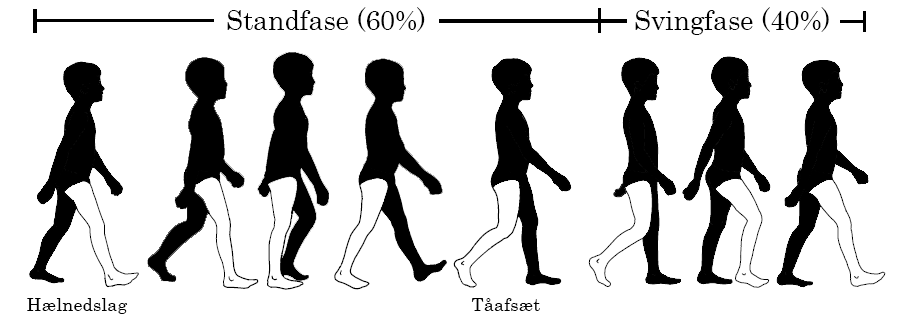
\includegraphics[scale=0.7]{figures/bProblemloesning/gang_cyklus.png}
	\caption{På figuren ses en gangcyklus, beskrevet for et ben, opdelt i henholdsvis en standfase og en svingfase. Standfasen udgør en større procentdel af den samlede cyklus end svingfasen. Ydermere indeholder standfasen cyklussens hælnedslag og tåafsæt. \citep{VaughanDavisOConnor1992} (Modificeret)}
	\label{fig:gang_cyklus}
\end{figure}
Følgende beskrivelse tager udgangspunkt i \figref{fig:gang_cyklus}. En gangcyklus inddeles i to faser; standfasen og svingfasen. Standfasens varighed er cirka 60\% af én gangcyklus og påbegyndes med den første dobbeltstøtte, hvilket sker, når den højre hæl opnår kontakt med underlaget. Efter dette placeres foden fladt på underlaget, hvor der er enkelt benstøtte, da venstre fod her hæves over jorden. Herefter opstår den anden dobbelt støtte, idet der opstår et hælslip med den højre fod. Samtidig med dette skabes en berøring af den venstre fod på underlaget som støtte i bevægelsen. Standfasen afsluttes med en dorsalfleksion af anklen og dermed et afsæt fra tæerne på højre fod. \citep{VaughanDavisOConnor1992,Whittle1990}  \newline 
Når højre fod og højre ben er i svingfasen, udgør dette cirka 40\% af én gangcyklus. Svingfasen påbegyndes med en acceleration af foden og benet, når foden ikke længere har kontakt med underlaget i standfasen. Den højre fod svinges fremad, hvorefter et såkaldt midt-sving forekommer, hvor højre fod er lige under kroppen. Afsluttende for svingfasen er der en deacceleration. Denne fase involverer benets muskulatur, som sænker hastigheden af benets og fodens fremadgående bevægelse. Derved er kroppen klar til det kommende hælnedslag, som initierer standfasen.\fxnote{herefter gentages cyklussen} \citep{VaughanDavisOConnor1992,Whittle1990}

De to faser beskrives altså i retningerne af henholdsvis x- og y-aksen. \Figref{fig:kraefter_akser} viser den kraftpåvirkning, som eksempelvis forekommer ved et hælnedslag i begge akser.  
\begin{figure}[H]
	\centering
	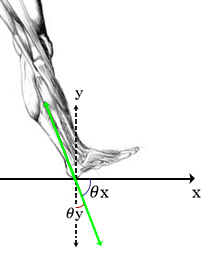
\includegraphics[scale=0.7]{figures/bProblemloesning/kraefter_akser.png}
	\caption{På figuren ses kraftpåvirkningerne for x- og y-aksen ved et hælnedslag. Den totale kraftpåvirkning ved hælnedslag er indikeret med en pil. Denne har en mindre vinkel til y-aksen, hvormed kraftpåvirkningen i y-aksens retning er størst.}
	\label{fig:kraefter_akser}
\end{figure} %Standfasens begyndelse og afslutning, med hælnedslag og tåafsæt, har størst kraftpåvirkning i y-aksens retning, idet foden henholdsvis sættes i jorden og løftes op igen uden betydelig bevægelse i x-aksens retning. Derimod har svingfasen størst kraftpåvirkning i x-aksens retning, da foden og benet, efter at være blevet hævet fra jorden, føres frem og initierer et nyt hæl-nedslag. I denne fase sker der ligeledes en bevægelse i y-aksens retning af mindre betydning. \citep{Rueterbories2010}
\Figref{fig:kraefter_akser} illustrerer den resulterende krafts retning i forbindelse med et hælnedslag. Yderligere fremgår det, at vinklen mellem den resulterende kraft og y-aksen er mindre end vinklen mellem x-aksen og den resulterende kraft. Kraftpåvirkningen i forbindelse med et hælnedslag er altså størst i y-aksens retning og derfor mest karakteristisk. Det beskrevne tilfælde for kraftpåvirkning i y-aksen i forbindelse med hælnedslag er ligeledes gældende for hele gangcyklussens faser. \citep{Rueterbories2010,Serway2010,ClelandKikhia2013}
%Hælnedslag og tåafsæt vil ydermere være særligt fremtrædende på y-aksen for et accelerometer, hvilket fremgår af \figref{fig:kraefter_akser}. Et eksempel på et gangsignal optaget med accelerometerets y-akse kan ses på \figref{fig:gang_y_acc}. 
%\begin{figure}[H]
%	\centering
%	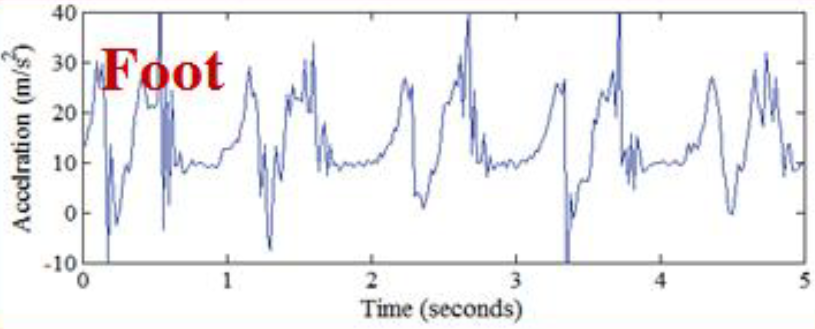
\includegraphics[scale=0.7]{figures/bProblemloesning/gang_y_acc.png}
%	\caption{På billedet ses et gangsignal optaget med accelerometerets y-akse. \citep{ClelandKikhia2013} (Modificeret)}
%	\label{fig:gang_y_acc}
%\end{figure}
%Figuren illustrerer en kraftpåvirkning i y-aksens retning ved de pågældende faser. Der forekommer to karakteristiske peaks ved y-aksen henholdsvis for hælnedslag og tåafsæt. Disse peaks kan derfor være fordelagtige at benytte til at undersøge accelerometerets data fra y-aksen i forhold til algoritmedesign. %, men henhold til hvorvidt sensoren har detekteret en gang-cyklus. 

\subsection{Løb}
Løb er en fysisk aktivitet, som er kendetegnet ved, at maks én fod rører jorden af gangen. Aktiviteten er en hurtigere version af gang og beskrives ligeledes som en cyklus men indeholder dog fire faser, som det ses på \figref{fig:loebecyklus}: standfasen, den første svævefase, svingfasen og den anden svævefase. \citep{Adelaar1986,Novacheck1998}
\begin{figure}[H]
	\centering
	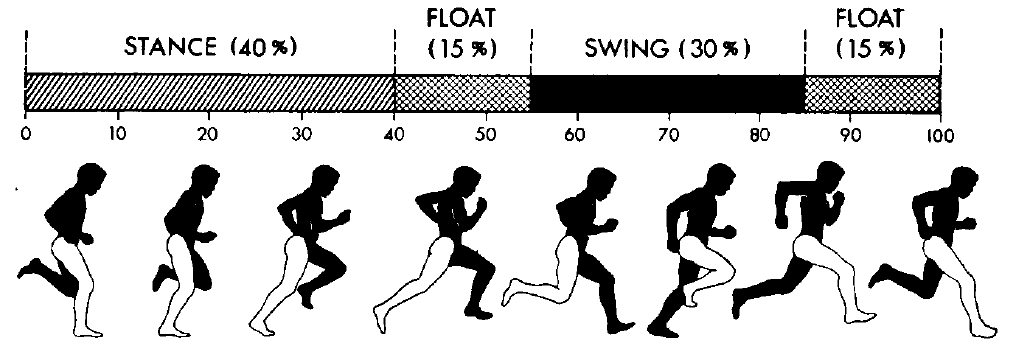
\includegraphics[scale=0.4]{figures/bProblemloesning/loeb_cyklus1.png}
	\caption{På figuren ses en løbecyklus opdelt i standfase, svingfase og to svævefaser. Standfasen udgør en minimalt større procentdel af cyklussen i forhold til svingfasen. Yderligere fremkommer svævefaserne ved løb. \citep{Adelaar1986} (Modificeret)}
	\label{fig:loebecyklus}
\end{figure}
Følgende beskrivelse tager udgangspunkt i \figref{fig:loebecyklus}. På samme vis som ved gangcyklussen begynder løbecyklussen idet øjeblik, hvor højre hæl rammer jorden. Dette er begyndelsen af standfasenen, som udgør 40\% af løbecyklussen. Herefter fortsætter foden til midtstand, hvor den er fladt placeret på jorden. Afslutningsvis udføres et accelererende afsæt med tæerne, som leder op til den næste fase, der er den første svævefase. \citep{Adelaar1986,Novacheck1998} \newline 
De to svævefaser, som findes to gange i løbecyklussen, er identiske og udgør hver især 15\% af cyklussen. Disse er karakteriseret ved, at begge ben er løftet fra jorden. \citep{Adelaar1986,Novacheck1998} Svævefasen begynder idet, at tåafsættet har løftet foden fra jorden. Mellem de to svævefaser er svingfasen, som udgør 30\% af løbecyklussen. Denne fase indebærer, at foden hæves og knæet føres frem, hvorefter hælen igen sænkes. Dette sker, mens den venstre fod udfører standfasen, hvorved højre fods svingfase er støttet af den venstre fod i jorden. \citep{Adelaar1986,Novacheck1998} %Efter denne svævefase fase udføres anden svævefase før en ny cyklus kan påbegyndes. 

Ved løb er maks én fod i kontakt med jorden ad gangen, hvilket resulterer i at der er et større stress på leddene ved løb i forhold til gang. Eksempelvis vil en person på 68 kilogram (kg) have et stress på sin fod på 35 kg/m ved gang, mens der ved løb vil være et stress på 110.000 kg/m. Kraftpåvirkningen er derfor ligeledes større ved løb. \citep{Adelaar1986} Dette suppleres af kraftpåvirkningen i de forskellige retninger under både gang og løb, hvor faserne domineres forskelligt af kraftpåvirkning i x- og y-aksens retning. \newline 
Standfasens hælnedslag og tåafsæt under gang og løb  er særligt karakteristisk grundet sin kraftpåvirkning i y-aksens retning. Kraftpåvirkningen er dog større ved løb, da denne fase ikke er understøttet af venstre fod. Kraftpåvirkningen i x-aksens retning for standfasen er af mindre betydning, da foden sættes i jorden og løftes op igen.\fxnote{Denne er større ved løb end gang, da hæl-nedslaget, som det ses på \figref{fig:loebecyklus}, er mere skråt på/har en mindre vinkel i forhold til jordoverfladen.} Modsat har svingfasen under gang og løb størst kraftpåvirkning i x-aksens retning, da accelerationen fremad af knæ og fod påvirker x-aksen mere end y-aksen. \citep{Rueterbories2010} 

\subsection{Cykling}
Cykling er en aktivitetsform, der udnytter kraftoverførslen mellem en person og en cykel. For at opnå en fremdrift af cyklen benytter brugeren hovedsageligt en statisk position af overkroppen, hvorimod de nedre lemmer udfører kraftudviklingen. \citep{Springer2014} Kraftoverførslen forekommer ved, at brugeren belaster cyklens pedaler, som er påsat cyklens krank. De roterende bevægelser med de nedre ekstremiteter skaber en fremdrift i hele systemet. Bevægelserne er opdelt i to lige lange faser; en kraftudøvende- og en restituerende fase, hvilket fremgår af \figref{fig:cykel_cyklus}.
\begin{figure}[H]
	\centering
	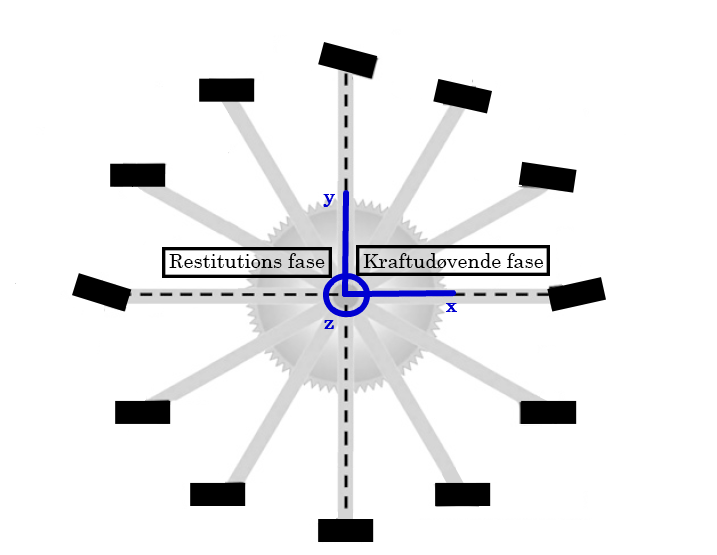
\includegraphics[scale=0.45]{figures/bProblemloesning/cykel_cyklus.png}
	\caption{På figuren ses cyklussen for cykling, som er opdelt to faser; en kraftudøvende- og en restituerende fase. Ydermere ses kraftpåvirkningen på pedalen i forskellige placeringer. \citep{Springer2014} (Modificeret)}
	\label{fig:cykel_cyklus}
\end{figure}
Det fremgår af ovenstående figur, at cykling er en bevægelse af de nedre ekstremiteter, som påvirker både x- og y-aksen. Der er dog tale om en cirkulær bevægelse om z-aksen. Idet cykling udføres i en cirkulær bevægelse vil det være muligt at bestemme det antal grader, som benet har roteret om den pågældende akse. Derfor har en række studier beskrevet, at cykling med fordel kan detekteres af et gyroskop, som kan måle vinkelændringen af et bens bevægelse rundt om en akse. Dermed vil gyroskopets output i en cyklus for cykling under ideelle forhold være tilsvarende en sinus kurve. \citep{Cockcroft2011,Marin-PerianuMarin-Perianu2013} 


\subsection{Karakteristika for de tre aktivitetsformer}
En gangcyklus og løbecyklus er blandt andet karakteriseret ved at have en kraftpåvirkning i y-aksens retning ved hælnedslag og tåafsæt. Et eksempel på disse to kraftpåvirkninger i y-aksens retning kan ses under løb på \figref{fig:loeb_skolebog}. Signalet for gang vil til dels ligne dette signal dog med forskel på varigheden af henholdsvis stand- og svingfasen. Dette skyldes, at standfasen reduceres i varighed for løb i forhold til gang. %Som de nævnes i \secref{acc_og_gyro} er et gyro bedst til at detektere alle de tre aktivitetsformer. Gyrtoskopet bruger meget strøm, og et accelerometer som kan bestemme kraftpåvirkningen i y-aksens retning vil derfor være fordelagtigt at benytte. \citep{Lee1998,Rueterbories2010}
\begin{figure}[H]
	\centering
	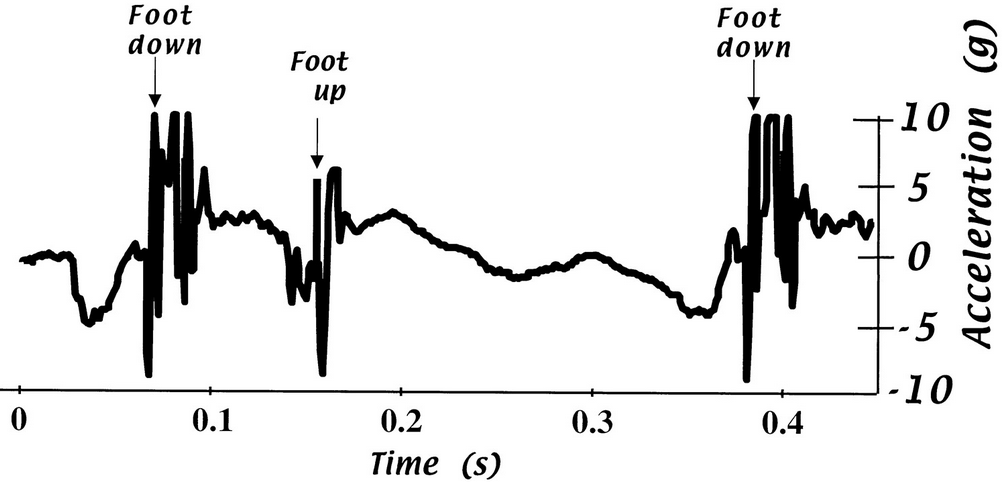
\includegraphics[scale=0.3]{figures/bProblemloesning/loeb_skolebog.png}
	\caption{På figuren ses et signal for løb optaget med et accelerometer, der er placeret på anklen. Accelerationen, på y-aksen, fremgår som funktion af tiden på x-aksen. En cyklus er angivet med den tilhørende stand- og svingfase. Ydermere er hælnedslag markeret med et blåt kryds, og et tåafsæt er markeret med en gul cirkel. \citep{WeyandKelly2001} (Modificeret)}
	\label{fig:loeb_skolebog}
\end{figure}
En cykelcyklus har ikke nogen væsentlig acceleration i vertikal eller horisontal retning men derimod rotation om én akse. Måling med et gyroskop vil dermed repræsentere ændringerne i vinklen om aksen. \citep{Cockcroft2011,Marin-PerianuMarin-Perianu2013}
%En cykelcyklus har dog ikke nogen væsentlig acceleration i vertikal eller horisontal retning, hvormed et accelerometer ikke er optimalt til detektering af cykling. Ved en cykelcyklus benyttes der cirkulære bevægelser om én akse, hvormed de cirkulære bevægelser vil repræsentere den i ændring i vinkler som forekommer. Derfor vil et gyropskop være fordelagtigt at benytte til detekteringen af cykling. \citep{Cockcroft2011,Marin-PerianuMarin-Perianu2013}


%De tre forskellige aktivitetsformer har flere fællestræk, men også en række karakteristika som adskiller dem fra hinanden. \newline 
%Gang er en aktivitet karakteriseret som en cyklus, hvor der altid er én eller to fødder i jorden. Denne cyklus er udgjort af to faser, en standfase og en svingfase, som hver udgør henholdsvis 60\% og 40\%.
%%Faserne for højre og venstre fod er identiske, men forskudt med en halv cyklus, hvilket resulterer i at standfasen for højre og venstre fod overlappes. Herved vil personen to gange i cyklussen have begge fødder i jorden samtidig. \newline
%kraftpåvirkningen under faserne domineres i forskellige retninger. Under standfasen domineres den primært i y-aksens retning, mens den i svingfasen primært domineres i x-aksens retning.
%
%Løb er i grundtræk meget lignende gang, blot hurtigere; fod- og benbevægelser er ens for gangcyklussen og løbecyklussen. Da løb går betydelig hurtigere er der i denne cyklus to faser, svævefaser, som ikke optræder ved gang, hvor begge fødder er hævet fra jorden. Standfasen og svingfasen er derfor kortere ved løb og udgør henholdsvis 40\% og 30\%, mens de to svævefaser hver udgør 15\%. \newline
%I denne fase er der ikke altid en fod i jorden, og det er maksimalt én fod i jorden ad gangen, hvilket gør at en person vil have et større stress på foden når hælen isættes i starten af standfasen sammenlignet med gang, hvor der altid er en fod i jorden. Dette stress vil i denne fase primært være påvirket af en kraftpåvirkning i y-aksens retning, mens kraftpåvirkningen under svingfasen domineres i x-aksens retning.
%
%Hvis hastigheden øges til en spurt i stedet for løb, er cyklussen den samme, dog ændres længden af faserne. Standfasen og svingfasen reduceres mens svævefaserne øges. \citep{Lee1998}\fxnote{Opg: Skal vi have mere om dette, det virker måske lidt kort.}
%
%Cykling adskiller sig betydeligt mere fra gang og løb, da denne er en roterende cyklus, som er opdelt i to lige lange faser, en kraftudøvende- og en restituerende fase. Under de to faser udfører fødderne og benene en cirkulær bevægelse, som roterer omkring en z-akse, hvorfor det repræsentativt kan måles med et gyroskop. 
